% Copyright (c) 2022 by Lars Spreng
% This work is licensed under the Creative Commons Attribution 4.0 International License.
 
\documentclass[
11pt,notheorems,hyperref={pdfauthor=whatever}
]{beamer}
 
% --- XeLaTeX 사용: fontenc/inputenc는 불필요 (있어도 무시되지만 제거 권장) ---
\usepackage{kotex}
 
\input{loadslides.tex}
 
% ============================================================================
% Korean font setup for XeLaTeX + Beamer
% 문제: helvet(sans-serif=Helvetica) + kotex 조합에서 한글 fallback이 안 되어
%       PDF에 한글이 빠짐 ("Missing character: There is no 미..." 경고).
% 해결: 한글 sans 폰트를 명시적으로 지정 + Beamer는 sans 기본이므로 sf default.
% ============================================================================
\usepackage{fontspec}
% Font discovery can be brittle under sandboxed XeLaTeX, so use the installed
% Noto CJK font files directly.
\setmainhangulfont[
    Path=/Users/seojunha/Library/Fonts/,
    BoldFont=NotoSansCJKkr-Bold.otf
]{NotoSansCJKkr-Regular.otf}
\setsanshangulfont[
    Path=/Users/seojunha/Library/Fonts/,
    BoldFont=NotoSansCJKkr-Bold.otf
]{NotoSansCJKkr-Regular.otf}
\setmonohangulfont[
    Path=/Users/seojunha/Library/Fonts/,
    BoldFont=NotoSansCJKkr-Bold.otf
]{NotoSansCJKkr-Regular.otf}
% Beamer 기본 sans -> 한글도 sans로 표시되게
\renewcommand{\familydefault}{\sfdefault}
% [폰트 못 찾을 때 대안]: 위 3줄을 지우고 아래로 교체
%   \setmainhangulfont{AppleMyungjo}
%   \setsanshangulfont{AppleGothic}
%   \setmonohangulfont{NanumGothicCoding}
% ============================================================================
 
\usepackage{tikz}
\usetikzlibrary{arrows.meta, positioning, fit, backgrounds}
 
% Reduce gap between frame title and content
\addtobeamertemplate{frametitle}{}{\vspace{-0.5em}}
 
\title[]{4/23 미팅}
\subtitle{MUSE 및 ACTMED 계산 방식 정리}
\author[]{하서준}
\institute{DGIST}
\date{\today}
 
\begin{document}


{
\setbeamertemplate{footline}{}
\begin{frame}
  \titlepage
\end{frame}
}
\addtocounter{framenumber}{-1}

% ─────────────────────────────────────────────────────────────────────────────
% FRAME 1: Initialization
% ─────────────────────────────────────────────────────────────────────────────
\begin{frame}{Initialization}
\begin{columns}[c]

\begin{column}{0.54\textwidth}

    \begin{block}{환자 노드 \quad $i = 1, \dots, B$}
    \[
        \mathbf{h}_i^{(0)} = \mathbf{1} \in \mathbb{R}^{d}
    \]
    \footnotesize
    모든 값이 1인 상수 벡터 ($d=128$). 직접 학습되지 않음.\\
    Message passing 및 노드 update 과정에서 값이 갱신됨.\\
    최종 노드 임베딩이 classification에 사용됨.
    \end{block}

    \vspace{0.1em}

    \begin{block}{Modality 노드 \quad $m \in \{1,2,3\}$}
    \[
        \mathbf{h}_m^{(0)} = \boldsymbol{\theta}_m \in \mathbb{R}^{d},
        \quad \boldsymbol{\theta}_m \sim \mathcal{N}(0,1)
    \]
    \footnotesize
    Modality 유형별로 하나의 학습 가능한 벡터. 모든 환자에서 공유됨.\\
    ``이 modality가 어떤 종류인가''를 표현함.\\
    \textcolor{gray}{(논문: OneHot($m$) $\in\mathbb{R}^3$;\; 코드: \texttt{nn.Parameter} $\in\mathbb{R}^{128}$)}
    \end{block}

    \vspace{0.1em}

    \begin{block}{Edge 속성 \quad (환자 $i$ $\leftrightarrow$ modality $m$)}
    \[
        \mathbf{e}_{im}^{(0)} = f_m(\mathbf{x}_i) \in \mathbb{R}^{d}
    \]
    \footnotesize
    Modality별 인코더 $f_m$ (FFN / RNN / Transformer)의 출력값.\\
    환자 $i$가 modality $m$을 보유한 경우(\texttt{flag}$_{im}=1$)에만 edge 존재.\\
    양방향 초기값 동일: $\mathbf{e}_{im}^{(0)} = \mathbf{e}_{mi}^{(0)}$
    \textcolor{gray}{(\texttt{repeat(2,1)}).}
    \end{block}

\end{column}

\begin{column}{0.42\textwidth}
    \centering
    \begin{tikzpicture}[
        pnode/.style={circle, draw=blue!60, fill=blue!10,
                      minimum size=0.72cm, font=\small, thick},
        mnode/.style={circle, draw=orange!80, fill=orange!15,
                      minimum size=0.72cm, font=\small, thick},
        every label/.style={font=\scriptsize},
        >=Stealth
    ]
        % patient nodes
        \node[pnode] (p1) at (0, 3.2) {$\mathbf{1}$};
        \node[pnode] (p2) at (0, 2.0) {$\mathbf{1}$};
        \node[pnode] (p3) at (0, 0.8) {$\mathbf{1}$};
        \node[left=0.05cm of p1, font=\scriptsize, blue!70] {$p_1$};
        \node[left=0.05cm of p2, font=\scriptsize, blue!70] {$p_2$};
        \node[left=0.05cm of p3, font=\scriptsize, blue!70] {$p_3$};

        % modality nodes
        \node[mnode] (m1) at (3.2, 3.0) {$\boldsymbol{\theta}_1$};
        \node[mnode] (m2) at (3.2, 2.0) {$\boldsymbol{\theta}_2$};
        \node[mnode] (m3) at (3.2, 1.0) {$\boldsymbol{\theta}_3$};
        \node[right=0.05cm of m1, font=\scriptsize, orange!80] {$m_1$};
        \node[right=0.05cm of m2, font=\scriptsize, orange!80] {$m_2$};
        \node[right=0.05cm of m3, font=\scriptsize, orange!80] {$m_3$};

        % edges
        \draw[<->, thick, gray!70] (p1) -- node[above, font=\tiny, sloped]{$f_1(\mathbf{x}_1)$} (m1);
        \draw[<->, thick, gray!70] (p1) -- (m2);
        \draw[<->, thick, gray!70] (p2) -- (m1);
        \draw[<->, thick, gray!70] (p2) -- (m3);
        \draw[<->, thick, gray!70] (p3) -- (m2);
        % p3--m1 missing

        \node[font=\tiny, red!60] at (1.3, 0.2) {(edge 없음 $=$ modality 누락)};

        % legend
        \node[pnode, minimum size=0.35cm] (lp) at (0.3, -0.4) {};
        \node[right=0.05cm of lp, font=\tiny] {환자 노드};
        \node[mnode, minimum size=0.35cm] (lm) at (0.3, -0.9) {};
        \node[right=0.05cm of lm, font=\tiny] {Modality 노드};
    \end{tikzpicture}
\end{column}

\end{columns}
\end{frame}


% ─────────────────────────────────────────────────────────────────────────────
% FRAME 2: Message Passing
% ─────────────────────────────────────────────────────────────────────────────
\begin{frame}{Message Passing (1 Hop)}
\begin{columns}[c]

\begin{column}{0.54\textwidth}

    \begin{block}{1.\ Message 생성 \quad ($d \to d$)}
    {\small\[
        \mathbf{msg}_{j \to i}^{(l)}
        = \text{ReLU}\!\left(
            \mathbf{W}^{(l)} \mathbf{h}_j^{(l-1)}
            + \mathbf{O}^{(l)} \mathbf{e}_{ji}^{(l-1)}
        \right) \in \mathbb{R}^d
    \]}
    \footnotesize
    Edge마다 독립적으로 message 생성:\\
    송신 노드 $\mathbf{h}_j$ + 해당 edge 속성 $\mathbf{e}_{ji}$ → concat → Linear → ReLU.
    \end{block}

    \begin{block}{2.\ Aggregation \quad ($d \to d$)}
    {\small\[
        \mathbf{a}_i^{(l)}
        = \frac{1}{|\mathcal{N}(i)|}
          \sum_{j \in \mathcal{N}(i)} \mathbf{msg}_{j \to i}^{(l)} \in \mathbb{R}^d
    \]}
    \footnotesize
    이웃 $\mathcal{N}(i)$로부터 수신된 message를 mean pooling.\\
    연결 구조에 따라 수신 message 수가 달라지며,\\
    집계값은 다음 node update의 입력으로 사용됨.
    \end{block}

    \begin{block}{3.\ Update \quad ($2d \to d$, Eq.\ 7)}
    {\small\[
        \mathbf{h}_i^{(l)}
        = \text{ReLU}\!\left(\mathbf{U}^{(l)}
          \underbrace{\text{Concat}\!\left(\mathbf{h}_i^{(l-1)},\ \mathbf{a}_i^{(l)}\right)}_{\in\,\mathbb{R}^{2d}}\right) \in \mathbb{R}^d
    \]}
    \footnotesize
    이전 자신의 임베딩 + aggregated 이웃 정보를 결합.
    \textbf{모든 노드에 동시에}, \textbf{양방향으로} 적용됨.
    \end{block}

\end{column}

\begin{column}{0.42\textwidth}
    \centering
    \begin{tikzpicture}[
        pnode/.style={circle, draw=blue!60, fill=blue!10,
                      minimum size=0.72cm, font=\small, thick},
        mnode/.style={circle, draw=orange!80, fill=orange!15,
                      minimum size=0.72cm, font=\small, thick},
        >=Stealth
    ]
        \node[pnode] (p1) at (0, 3.4) {$p_1$};
        \node[pnode] (p2) at (0, 1.6) {$p_2$};
        \node[mnode] (m1) at (3.2, 2.5) {$m_1$};

        \draw[->, thick, blue!60, bend left=15]
            (p1) to node[above, sloped, font=\tiny]{msg} (m1);
        \draw[->, thick, blue!60, bend right=15]
            (p2) to node[below, sloped, font=\tiny]{msg} (m1);
        \draw[->, thick, orange!70, bend right=15]
            (m1) to node[above, sloped, font=\tiny]{msg} (p1);
        \draw[->, thick, orange!70, bend left=15]
            (m1) to node[below, sloped, font=\tiny]{msg} (p2);

        \node[draw=orange!50, fill=orange!5, rounded corners,
              font=\tiny, text width=2.2cm, align=center]
            at (3.2, 0.8)
            {$p_1$, $p_2$ message\\mean pooling\\
             \textcolor{gray!70}{동시 node update}};
        \draw[->, dashed, orange!50] (3.2, 1.15) -- (m1);
    \end{tikzpicture}

    \vspace{0.6em}
    \begin{tikzpicture}
    \node[draw=gray!40, rounded corners, fill=gray!5,
          font=\scriptsize, text width=4.2cm]{
        \textbf{1-hop}: 연결된 이웃으로부터\\
        \quad message를 수신하고 집계\\[0.3em]
        \textbf{2-hop}: 갱신된 노드/edge 상태로\\
        \quad 동일 연산을 반복\\[0.3em]
        \textcolor{gray}{단일 환자 추론에서도 동일한 계산 흐름}
    };
    \end{tikzpicture}
\end{column}

\end{columns}
\end{frame}


% ─────────────────────────────────────────────────────────────────────────────
% FRAME 3: Edge Update
% ─────────────────────────────────────────────────────────────────────────────
\begin{frame}{Edge Update}
\begin{columns}[c]

\begin{column}{0.52\textwidth}

    \textbf{각 hop 완료 후} (마지막 hop 제외), 모든 edge 속성 갱신:
    \[
        \mathbf{e}_{ji}^{(l)}
        = \text{ReLU}\!\left(\mathbf{P}^{(l)}
          \underbrace{\text{Concat}\!\left(
            \mathbf{h}_j^{(l)},\ \mathbf{h}_i^{(l)},\ \mathbf{e}_{ji}^{(l-1)}
          \right)}_{\in\,\mathbb{R}^{3d}}\right) \in \mathbb{R}^d
    \]
    \footnotesize
    업데이트된 송신/수신 노드 임베딩
    $\mathbf{h}_j^{(l)}, \mathbf{h}_i^{(l)}$과 이전 edge 속성
    $\mathbf{e}_{ji}^{(l-1)}$을 concat하여 새 edge 속성 생성.

    \vspace{0.5em}
    \normalsize
    \begin{itemize}\itemsep0.3em
        \item 방향이 바뀌면 concat 입력의 송신/수신 순서도 달라짐\\
              \footnotesize $\text{Concat}(\mathbf{h}_j^{(l)},\mathbf{h}_i^{(l)},\mathbf{e}_{ji}^{(l-1)})$
        \normalsize
        \item 갱신된 edge 속성은 \textbf{다음 hop의} message 생성에 입력으로 사용됨
    \end{itemize}

    \vspace{0.4em}
    \begin{tikzpicture}
    \node[draw=gray!40, rounded corners, fill=gray!5,
          font=\scriptsize, text width=5.2cm]{
        \textbf{초기 (hop 0)}: 양방향 edge에 동일한 modality encoder 출력 사용\\[0.3em]
        \textbf{edge update 이후}: 방향별 입력 순서에 따라 별도 edge state 유지
    };
    \end{tikzpicture}

\end{column}

\begin{column}{0.44\textwidth}
    \centering
    \begin{tikzpicture}[
        pnode/.style={circle, draw=blue!60, fill=blue!10,
                      minimum size=0.80cm, font=\small, thick},
        mnode/.style={circle, draw=orange!80, fill=orange!15,
                      minimum size=0.80cm, font=\small, thick},
        >=Stealth
    ]
        \node[pnode] (p) at (0, 2.2) {$p_i$};
        \node[mnode] (m) at (4.0, 2.2) {$m_j$};

        \draw[->, bend left=30, thick, blue!60]
            (p) to node[above, font=\scriptsize]{$\mathbf{e}_{ij}^{(l)}$} (m);
        \draw[->, bend left=30, thick, orange!70]
            (m) to node[below, font=\scriptsize]{$\mathbf{e}_{ji}^{(l)}$} (p);

        \node[font=\scriptsize, text width=3.8cm, align=center,
              draw=gray!30, rounded corners, fill=gray!5]
            at (2.0, 0.35)
            {반대 방향에 대해\\각각 \textbf{별도의} edge 벡터 존재};
    \end{tikzpicture}

\end{column}

\end{columns}
\end{frame}

% ─────────────────────────────────────────────────────────────────────────────
% FRAME 4: Modality Encoder
% ─────────────────────────────────────────────────────────────────────────────
\begin{frame}{MUSE의 Modality Encoder}

\begin{table}[]
\centering
\begin{tabular}{llll}
\toprule
\textbf{Modality} & \textbf{입력} & \textbf{Encoder} & \textbf{출력} \\
\midrule
의료 코드 & ICD 진단/시술/ & Transformer & \multirow{2}{*}{128차원} \\
          & 처방 코드 ID & (처음부터 학습) & \\
\midrule
검사 수치  & 114개 검사 항목 & 양방향 & \multirow{2}{*}{128차원} \\
          & 시계열 데이터  & GRU    & \\
\midrule
임상 노트 & 퇴원 요약문 & Bio\_ClinicalBERT & \multirow{2}{*}{128차원} \\
          &            & (frozen)         & \\
\bottomrule
\end{tabular}
\end{table}

\vspace{0.5em}

\begin{block}{주요 설계 선택}
\begin{itemize}
    \item 코드 임베딩은 Bio\_ClinicalBERT로 인코딩된 코드 설명으로 초기화 (frozen lookup)
    \item 임상 노트 encoder는 완전히 frozen; 코드 Transformer는 end-to-end로 fine-tuning
    \item 모든 modality는 GNN 입력 전에 동일한 128차원 공간으로 투영됨
\end{itemize}
\end{block}

\end{frame}

% ─────────────────────────────────────────────────────────────────────────────
% FRAME 5: Batch Size and Graph Size
% ─────────────────────────────────────────────────────────────────────────────
\begin{frame}{Batch 크기에 따라 Bipartite Graph 크기 변화}
\begin{columns}[c]

\begin{column}{0.45\textwidth}
    \begin{block}{Batch당 그래프 구조}
    \begin{itemize}
        \item \textbf{환자 노드}: $B$개 (= batch 크기)
        \item \textbf{Modality 노드}: 3개 (고정)
        \item \textbf{Edge}: 최대 $3B$개 (보유 modality당 1개)
    \end{itemize}
    \end{block}

    \vspace{0.5em}

    \begin{tikzpicture}
    \node[draw=gray!40, rounded corners, fill=gray!5,
          font=\scriptsize, text width=5.0cm]{
        \textbf{Batch 크기 = 1} \quad $\Rightarrow$ 환자 노드 1개\\[0.3em]
        \textbf{Batch 크기 = 512} $\Rightarrow$ 환자 노드 512개\\[0.3em]
        Modality 노드는 항상 \textbf{3개} 고정\\[0.3em]
        $\therefore$ Batch 크기에 따라 graph 크기와\\
        \quad modality 노드의 aggregation 대상 수가 달라짐
    };
    \end{tikzpicture}
\end{column}

\begin{column}{0.52\textwidth}
\centering
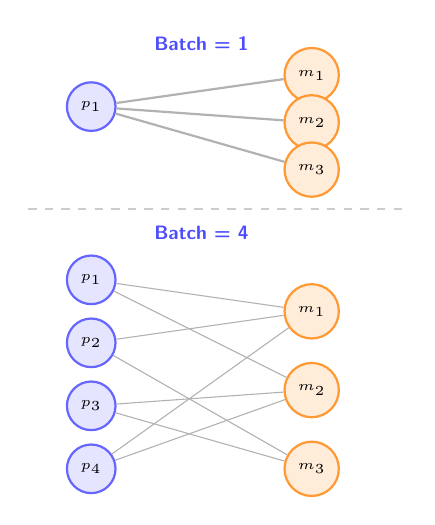
\begin{tikzpicture}[
    pnode/.style={circle, draw=blue!60, fill=blue!10,
                  minimum size=0.55cm, font=\tiny, thick},
    mnode/.style={circle, draw=orange!80, fill=orange!15,
                  minimum size=0.55cm, font=\tiny, thick},
    >=Stealth
]

% --- batch=1 (top) ---
\node[font=\scriptsize\bfseries, blue!70] at (2.2, 5.2) {Batch = 1};
\node[pnode] (b1p1) at (0.8, 4.4) {$p_1$};
\node[mnode] (b1m1) at (3.6, 4.8) {$m_1$};
\node[mnode] (b1m2) at (3.6, 4.2) {$m_2$};
\node[mnode] (b1m3) at (3.6, 3.6) {$m_3$};
\draw[gray!60, thick] (b1p1) -- (b1m1);
\draw[gray!60, thick] (b1p1) -- (b1m2);
\draw[gray!60, thick] (b1p1) -- (b1m3);

% divider
\draw[dashed, gray!40] (0, 3.1) -- (4.8, 3.1);

% --- batch=4 (bottom) ---
\node[font=\scriptsize\bfseries, blue!70] at (2.2, 2.8) {Batch = 4};
\node[pnode] (b4p1) at (0.8, 2.2) {$p_1$};
\node[pnode] (b4p2) at (0.8, 1.4) {$p_2$};
\node[pnode] (b4p3) at (0.8, 0.6) {$p_3$};
\node[pnode] (b4p4) at (0.8,-0.2) {$p_4$};
\node[mnode] (b4m1) at (3.6, 1.8) {$m_1$};
\node[mnode] (b4m2) at (3.6, 0.8) {$m_2$};
\node[mnode] (b4m3) at (3.6,-0.2) {$m_3$};
\draw[gray!60] (b4p1) -- (b4m1);
\draw[gray!60] (b4p1) -- (b4m2);
\draw[gray!60] (b4p2) -- (b4m1);
\draw[gray!60] (b4p2) -- (b4m3);
\draw[gray!60] (b4p3) -- (b4m2);
\draw[gray!60] (b4p3) -- (b4m3);
\draw[gray!60] (b4p4) -- (b4m1);
\draw[gray!60] (b4p4) -- (b4m2);

\end{tikzpicture}
\end{column}

\end{columns}
\end{frame}

% ─────────────────────────────────────────────────────────────────────────────
% FRAME 6: Experiment 1
% ─────────────────────────────────────────────────────────────────────────────
\begin{frame}{Experiment : Batch 크기가 추론 성능에 미치는 영향}
    \begin{figure}
        \centering
        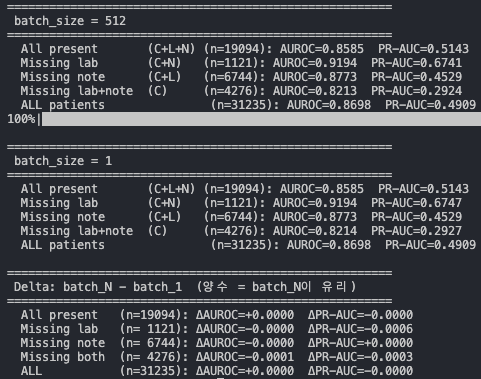
\includegraphics[width=0.5\linewidth]{result.png}
        \caption{Batch 크기에 따른 테스트셋 성능 (MIMIC-IV, 사망률 예측)}
        \label{fig:batch_effect}
    \end{figure}
    \begin{itemize}
        \item 동일한 checkpoint에서 batch 크기 512 vs.\ 1 비교 시
              $\Delta\text{AUROC} \approx 0.000$, $\Delta\text{PR-AUC} \approx 0.000$
              (모든 modality 누락 그룹에서 동일)

        \item \textbf{원인}: 환자 노드가 동일한 $\mathbf{1} \in \mathbb{R}^{d}$로 초기화되므로,
              환자들이 modality 노드로 보내는 message는
              edge 속성 $\mathbf{e}_{im}$의 batch 평균으로 수렴함.
              Batch 크기가 달라도 이 평균의 차이가 미미하여
              환자별 예측 \emph{순위}에 영향을 주지 못함.
              \textcolor{gray}{(AUROC는 순위 기반 지표)}

        \item MUSE는 단일 환자 추론 환경에서도
              \textbf{성능 저하 없음} $\Rightarrow$ 임상 배포 적합성 확인
    \end{itemize}
\end{frame}

% ─────────────────────────────────────────────────────────────────────────────
% ACTMED Section Title
% ─────────────────────────────────────────────────────────────────────────────
\begin{frame}[plain]
    \centering
    \vspace{2.0cm}
    {\Large\bfseries ACTMED}\\[0.8em]
    {\normalsize Active Test Selection for Timely Clinical Diagnosis}\\[0.5em]
    {\footnotesize Bayesian Experimental Design + LLM}
\end{frame}

% ─────────────────────────────────────────────────────────────────────────────
% FRAME 1: 문제 제기 - 임상 현실
% ─────────────────────────────────────────────────────────────────────────────
\begin{frame}{현실에서의 임상 진단}
\begin{columns}[c]

\begin{column}{0.48\textwidth}
    \begin{block}{진단은 정적 분류가 아님}
    \begin{itemize}\itemsep0.4em
        \item 진단은 본질적으로 \textbf{순차적}이고 \textbf{단계적}
        \item 환자 정보가 한 번에 모두 주어지지 않음
        \item 새 검사 결과에 따라 다음 판단이 계속 바뀜
    \end{itemize}
    \end{block}

    \vspace{0.4em}

    \begin{block}{검사는 공짜가 아님}
    \begin{itemize}\itemsep0.4em
        \item 검사마다 비용, 시간, 환자 부담 발생
        \item 불필요한 검사가 전체의 \textbf{40--60\%}로 추정
        \item WHO: 2035년까지 의료인력 \textbf{1,200만 명} 부족
    \end{itemize}
    \end{block}
\end{column}

\begin{column}{0.48\textwidth}
    \centering
    {\bfseries 동적 진단}\\[-0.1em]
    {\scriptsize\textcolor{gray}{현재 정보에 따라 검사 선택과 belief 업데이트를 반복}}\\[0.35em]
    \begin{tikzpicture}[
        diagstep/.style={draw=blue!45, fill=blue!5, rounded corners,
                         font=\scriptsize, text width=4.3cm, align=center,
                         minimum height=0.75cm},
        obs/.style={draw=orange!65, fill=orange!8, rounded corners,
                    font=\scriptsize, text width=4.3cm, align=center,
                    minimum height=0.75cm},
        >=Stealth
    ]
        \node[diagstep] (k) at (0, 3.2) {현재 정보 $K_t$\\증상, 병력, 기존 검사};
        \node[obs] (u) at (0, 2.1) {다음 검사 선택\\무엇을 더 볼 것인가?};
        \node[obs] (r) at (0, 1.0) {실제 검사 결과 관찰\\새 evidence 획득};
        \node[diagstep] (b) at (0, -0.1) {진단 belief 업데이트\\$K_{t+1}$로 이동};

        \draw[->, thick, gray!70] (k) -- (u);
        \draw[->, thick, gray!70] (u) -- (r);
        \draw[->, thick, gray!70] (r) -- (b);
        \draw[->, thick, dashed, gray!60] (b.east) -- ++(0.6,0) |- node[pos=0.25, right, font=\tiny, gray] {repeat} (k.east);
    \end{tikzpicture}

    \vspace{0.7em}

    \begin{alertblock}{핵심 문제}
    \small
    정확한 진단뿐 아니라, \textbf{어떤 검사를 언제 시행할지}를 환자별로 결정해야 함.
    \end{alertblock}
\end{column}

\end{columns}
\end{frame}


% ─────────────────────────────────────────────────────────────────────────────
% FRAME 2: 문제 제기 - 기존 방법의 한계
% ─────────────────────────────────────────────────────────────────────────────
\begin{frame}{기존 방법의 한계}
\begin{columns}[c]

\begin{column}{0.48\textwidth}
    \begin{block}{기존 방법의 전형적 한계}
    \footnotesize
    \begin{tabular}{lccc}
        \toprule
        방법 & 순차적 & 개인 맞춤 & 투명성 \\
        \midrule
        Rule-based      & \textcolor{red}{\texttimes} & \textcolor{red}{\texttimes}  & \textcolor{green!60!black}{\checkmark} \\
        Classical ML    & \textcolor{red}{\texttimes} & \textcolor{red}{\texttimes}  & \textcolor{red}{\texttimes} \\
        Deep Learning   & \textcolor{red}{\texttimes} & \textcolor{red}{\texttimes}  & \textcolor{red}{\texttimes} \\
        Na\"ive LLM     & \textcolor{green!60!black}{\checkmark} & \textcolor{red}{\texttimes}  & \textcolor{red}{\texttimes} \\
        \textbf{ACTMED} & \textcolor{green!60!black}{\checkmark} & \textcolor{green!60!black}{\checkmark} & \textcolor{green!60!black}{\checkmark} \\
        \bottomrule
    \end{tabular}\\[0.3em]
    \textcolor{gray}{\tiny 대부분의 기존 방법은 위 세 가지 중 하나 이상을 충족하지 못함.}
    \end{block}

    \vspace{0.3em}

    \begin{tikzpicture}
    \node[draw=gray!45, fill=gray!8, rounded corners,
          font=\scriptsize, text width=5.35cm, align=left]{
        \textbf{비교 대상 간단 정리}\\[0.2em]
        \textbf{Rule-based}: 설명 가능, 개인화/순차성 약함\\
        \textbf{Classical ML / Deep Learning}: 전체 feature가 있다고 가정\\
        \textbf{Na\"ive LLM}: 직접 추천 가능, 선택 기준 불명확\\
        \textbf{ACTMED}: 순차적·개인맞춤·투명한 검사 선택
    };
    \end{tikzpicture}
\end{column}

\begin{column}{0.48\textwidth}
    \begin{alertblock}{정적 ML 가정의 문제}
    \small
    기존 ML 모델은 \textbf{모든 데이터가 주어진다고 가정}하고 진단을 \textbf{정적 분류 문제}로 다룸.\\[0.4em]
    실제 임상 추론의 순차적·자원 인식적 특성을 반영하기 어려움.
    \end{alertblock}

    \vspace{0.35em}

    \begin{block}{Na\"ive LLM의 문제}
    \footnotesize
    \begin{itemize}
        \item 확률적 추론이 약함
        \item 모든 환자에게 \textbf{동일한 검사} 추천 (개인화 불가)
        \item 블랙박스: 추론 과정 불투명
    \end{itemize}
    \end{block}

    \vspace{0.35em}

    \begin{block}{필요한 조건}
    \footnotesize
    \begin{itemize}\itemsep0.25em
        \item 환자별 현재 정보에 따라 다음 검사를 선택
        \item 검사 비용을 고려한 정보 획득 기준
        \item 선택 과정이 임상의에게 설명 가능
    \end{itemize}
    \end{block}
\end{column}

\end{columns}
\end{frame}


% ─────────────────────────────────────────────────────────────────────────────
% FRAME 2: 아이디어
% ─────────────────────────────────────────────────────────────────────────────
\begin{frame}{아이디어 (Figure 2)}
\centering
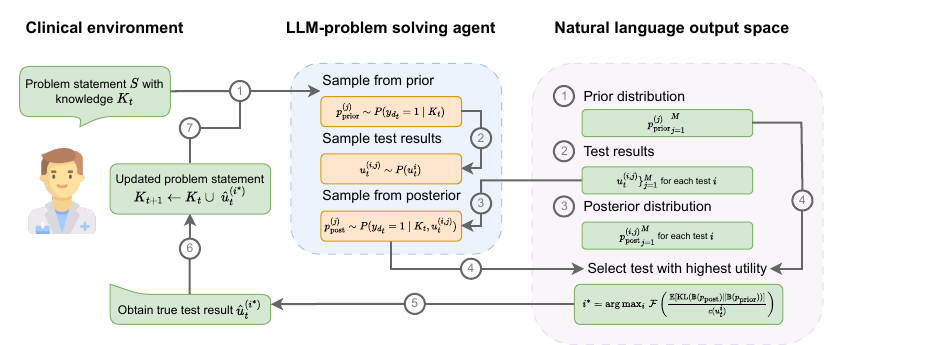
\includegraphics[width=0.92\textwidth]{figures/actmed_fig2_pipeline.png}

\vspace{0.5em}
\begin{columns}[t]
\begin{column}{0.31\textwidth}
\begin{block}{순차적 진단으로 재정의}
\footnotesize
진단을 한 번의 분류 문제가 아니라, 현재 정보 $K_t$에서 \textbf{다음 검사를 고르는} 의사결정 문제로 다룸.
\end{block}
\end{column}
\begin{column}{0.31\textwidth}
\begin{block}{각 검사별 기대 정보량 계산}
\footnotesize
각 후보 검사를 시행했을 때 진단 belief가 얼마나 바뀔지 미리 추정하고, 비용 대비 변화량이 큰 검사를 선택.
\end{block}
\end{column}
\begin{column}{0.31\textwidth}
\begin{block}{LLM을 서로게이트로 활용}
\footnotesize
복잡한 의료 분포를 직접 모델링하지 않고, LLM이 prior, 가상 검사 결과, posterior를 추정하도록 사용.
\end{block}
\end{column}
\end{columns}

\vspace{0.2em}
\footnotesize
\textcolor{gray}{ACTMED는 영상/텍스트/혈액 같은 modality 선택이 아니라, 관측할 \textbf{검사 항목(feature)}을 고르는 Active Feature Acquisition 문제.}
\end{frame}


% ─────────────────────────────────────────────────────────────────────────────
% FRAME 3: LLM의 역할
% ─────────────────────────────────────────────────────────────────────────────
\begin{frame}{LLM의 역할: 서로게이트 샘플러}
\begin{columns}[c]

\begin{column}{0.54\textwidth}

    \begin{block}{왜 수식 모델이 아닌가?}
    \footnotesize
    공학/물리학에서 BED는 닫힌 형태의 수식 사용.\\[0.3em]
    의료에서는: 생리학적 변수들이 \textbf{비선형, 고차원, 부분 관측}
    $\Rightarrow$ 직접 모델링 \textbf{불가}.
    \end{block}

    \vspace{0.3em}

    \begin{block}{LLM을 서로게이트로}
    \footnotesize
    LLM은 대규모 의학 문헌에서 의학 지식을 학습.\\[0.3em]
    $K_t$를 프롬프트로 받아 \textbf{조건부 샘플러}처럼 작동:
    \[
        u^{(i,j)}_t \sim P(U^{(i)}_t \mid K_t)
    \]
    \vspace{-0.2em}
    \scriptsize
    \textcolor{gray}{현재 정보 $K_t$가 주어졌을 때, 후보 검사 $i$의 가능한 $j$번째 결과를 샘플링한다는 의미.}
    \end{block}

    \vspace{0.3em}

    \begin{block}{환각(Hallucination) 완화}
    \footnotesize
    \begin{enumerate}\itemsep0.2em
        \item 구조화된 임상 요약문(vignette) 프롬프트
        \item 가능한 검사 결과를 하나로 고정하지 않고 \textbf{여러 후보값으로 샘플링}
        \item 질병 있음/없음 \textbf{양쪽 모두} 고려하도록 지시
            \textcolor{gray}{--- 한쪽 진단으로 성급히 고정되는 것을 완화}
    \end{enumerate}
    \end{block}

\end{column}

\begin{column}{0.42\textwidth}

    \begin{block}{LLM이 하는 세 가지}
    \footnotesize
    \begin{tabular}{ll}
        \toprule
        역할 & 출력 \\
        \midrule
        Prior 추정    & $p_{\text{prior}} \in [0,1]$ \\
        검사 결과 생성 & $u^{(i,j)}_t \in \mathbb{R}$ \\
        Posterior 추정 & $p_{\text{post}} \in [0,1]$ \\
        \bottomrule
    \end{tabular}
    \end{block}

    \vspace{0.4em}

    \begin{block}{검사 utility 계산}
    \footnotesize
    \begin{center}
    \resizebox{\linewidth}{!}{$
    \mathbb{E}[\mathrm{KL}]
    = \frac{1}{M}\sum_{j=1}^{M}
    \left[
    p^{(j)}_{\text{post}}\log\frac{p^{(j)}_{\text{post}}}{p_{\text{prior}}}
    + (1-p^{(j)}_{\text{post}})\log\frac{1-p^{(j)}_{\text{post}}}{1-p_{\text{prior}}}
    \right]
    $}
    \end{center}
    \vspace{-0.4em}
    \scriptsize
    \textcolor{gray}{각 샘플별 prior--posterior 변화량을 KL로 계산한 뒤 평균낸 값.}
    \end{block}

    \vspace{0.3em}

    \begin{alertblock}{주의}
    \footnotesize
    프레임워크 품질은 \textbf{LLM 품질에 완전 종속}.\\
    GPT-4o급 필요; 작은 모델은 실패.
    \end{alertblock}

\end{column}

\end{columns}
\end{frame}


% ─────────────────────────────────────────────────────────────────────────────
% FRAME 4: 핵심 아이디어
% ─────────────────────────────────────────────────────────────────────────────
\begin{frame}{핵심 아이디어}
\begin{columns}[c]

\begin{column}{0.40\textwidth}

    \begin{block}{핵심 아이디어}
    \footnotesize
    \textbf{Bayesian Experimental Design (BED)} + \textbf{LLM}을 결합하여 실제 임상 추론을 모방.\\[0.4em]
    LLM의 강점(의학 지식)으로 검사 결과를 시뮬레이션하고,\\
    BED의 수학적 엄밀성으로 최적 검사를 선택.
    \end{block}

    \vspace{0.25em}

    \begin{block}{베이지안 실험 설계}
    \footnotesize
    \textit{``비용 대비 가장 많은 정보를 주는 검사는?''}\\[0.3em]
    {\scriptsize\[
        F(U_t^{(i)}) =
        \frac{\mathbb{E}[\mathrm{KL}(\mathbb{B}(p_{\text{post}})\|\mathbb{B}(p_{\text{prior}}))]}{c(U_t^{(i)})}
    \]}
    \textbf{비용 대비 정보량}이 가장 큰 검사를 선택.
    \end{block}

    \vspace{0.25em}

    \begin{block}{LLM의 역할}
    \footnotesize
    \begin{itemize}
        \item 단순 classifier로 바로 쓰는 것이 \textbf{아님}
        \item 핵심 역할은 \textbf{검사 선택을 위한 서로게이트}
        \item $u^{(i,j)}_t \sim P(U^{(i)}_t \mid K_t)$ --- 태스크별 학습 불필요
    \end{itemize}
    \end{block}

\end{column}

\begin{column}{0.56\textwidth}
    \centering
    \textbf{ACTMED selects the next diagnostic test at each time step $t$}\\[0.35em]
    \resizebox{\linewidth}{!}{%
    \begin{tikzpicture}[
        actstep/.style={draw=blue!45, fill=blue!5, rounded corners,
                        font=\scriptsize, text width=7.6cm, align=left,
                        minimum height=0.88cm, inner xsep=0.30cm},
        sample/.style={draw=orange!75, fill=orange!8, rounded corners,
                       font=\scriptsize, text width=7.6cm, align=left,
                       minimum height=0.88cm, inner xsep=0.30cm},
        select/.style={draw=green!55!black, fill=green!6, rounded corners,
                       font=\scriptsize, text width=7.6cm, align=left,
                       minimum height=0.88cm, inner xsep=0.30cm},
        >=Stealth
    ]
        \node[actstep] (p) at (0, 5.0)
            {\textbf{1. Prior 초기화}\\[-0.05em]
             현재 환자 정보 $K_t$로 질병 risk $p_{\text{prior}}$ 추정};
        \node[sample] (u) at (0, 4.0)
            {\textbf{2. 후보 검사별 가상 결과 샘플링}\\[-0.05em]
             각 검사 $U_t^{(i)}$에 대해 가능한 결과를 여러 번 생성};
        \node[sample] (q) at (0, 3.0)
            {\textbf{3. 각 가상 결과에서 posterior 추정}\\[-0.05em]
             가상 결과를 추가했을 때 risk가 얼마나 바뀌는지 계산};
        \node[actstep] (kl) at (0, 2.0)
            {\textbf{4. 검사 utility 계산}\\[-0.05em]
             belief 변화량(KL)을 평균내고 검사 비용으로 정규화};
        \node[select] (sel) at (0, 1.0)
            {\textbf{5. 다음 검사 선택}\\[-0.05em]
             비용 대비 정보량이 가장 큰 검사 $i^*$ 선택};
        \node[select] (upd) at (0, 0.0)
            {\textbf{6. 실제 결과 관측 후 업데이트}\\[-0.05em]
             실제 검사 결과를 반영해 $K_{t+1}$로 넘어가며 반복};

        \draw[->, thick, gray!75] (p) -- (u);
        \draw[->, thick, gray!75] (u) -- (q);
        \draw[->, thick, gray!75] (q) -- (kl);
        \draw[->, thick, gray!75] (kl) -- (sel);
        \draw[->, thick, gray!75] (sel) -- (upd);
        \draw[->, thick, dashed, gray!60] (upd.east) -- ++(0.45,0) |- node[pos=0.25, right, font=\tiny, gray] {repeat} (p.east);
    \end{tikzpicture}}

    \vspace{0.35em}
    \begin{block}{핵심 포인트}
    \footnotesize
    LLM은 검사 선택 과정에서 \textbf{prior}, 후보 검사 결과, \textbf{posterior}를 추정하는 서로게이트이고,
    선택 자체는 기대 KL divergence를 비용으로 정규화한 $F(U_t^{(i)})$로 결정된다.
    \end{block}
\end{column}

\end{columns}
\end{frame}


% ─────────────────────────────────────────────────────────────────────────────
% FRAME 4: Posterior-based Selection
% ─────────────────────────────────────────────────────────────────────────────
\begin{frame}{Posterior 기반 검사 선택 기준 (Figure 1)}
\centering
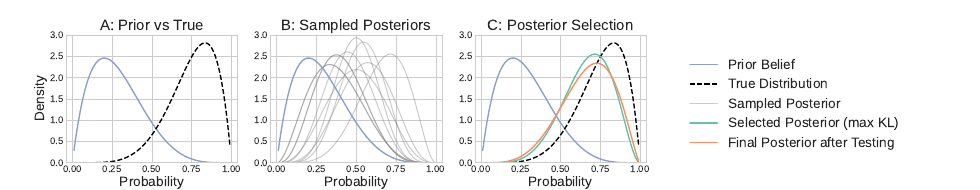
\includegraphics[width=0.99\textwidth]{figures/actmed_fig1_kl.png}

\vspace{0.55em}
\begin{columns}[t]
\begin{column}{0.31\textwidth}
\begin{block}{1.\ Prior belief}
\footnotesize
현재 정보 $K_t$만으로 질병 risk
$p_{\text{prior}}$를 먼저 추정.\\[0.25em]
\scriptsize
\textcolor{gray}{아직 새 검사를 보기 전의 현재 믿음.}
\end{block}
\end{column}
\begin{column}{0.31\textwidth}
\begin{block}{2.\ Posterior samples}
\footnotesize
후보 검사마다 결과를 $M=10$번 시뮬레이션하고,
각 결과별 $p_{\text{post}}^{(j)}$를 추정.\\[0.25em]
\scriptsize
\textcolor{gray}{각 검사별 가능한 결과 10개를 만들고, posterior 변화량을 평균.}
\end{block}
\end{column}
\begin{column}{0.31\textwidth}
\begin{block}{3.\ Utility}
\vspace{-0.9em}
\begin{center}
\resizebox{0.97\linewidth}{!}{$
F(U_t^{(i)}) =
\dfrac{\mathbb{E}[\mathrm{KL}(\mathbb{B}(p_{\text{post}})\|\mathbb{B}(p_{\text{prior}}))]}{c(U_t^{(i)})}
$}
\end{center}
\vspace{-0.75em}
\footnotesize
\raggedright
\textbf{평균 belief 변화량 / 비용}이\\
가장 큰 검사를 선택.\\[0.35em]
\scriptsize
\textcolor{gray}{불확실성 감소보다 ``진단 확률이 얼마나 바뀌는가''를 우선.}
\vspace{-0.1em}
\end{block}
\end{column}
\end{columns}

\vspace{0.9em}
\footnotesize
\textcolor{gray}{Figure 1은 Bernoulli PMF가 아니라, 후보 검사별 posterior risk가 prior에서 얼마나 이동하는지를 보여주는 개념도.}
\end{frame}


% ─────────────────────────────────────────────────────────────────────────────
% FRAME 6: 실험 설정
% ─────────────────────────────────────────────────────────────────────────────
\begin{frame}{실험 설정}
\begin{columns}[c]

\begin{column}{0.50\textwidth}

    \begin{block}{데이터셋}
    \footnotesize
    \begin{tabular}{llc}
        \toprule
        데이터셋 & 태스크 & 환자 수 \\
        \midrule
        CKD       & 신장 질환   & 157 \\
        Hepatitis & C형 간염    & 112 \\
        Diabetes  & 당뇨        & 100 \\
        OSCE      & 다중 질환   & 114$\times$2\textsuperscript{*} \\
        \bottomrule
    \end{tabular}\\[0.3em]
    \footnotesize
    \textsuperscript{*}실제 케이스 + 합성 음성 대조군\\
    모두 이진 분류, 구조화된 혈액 검사값만 사용\\
    $\Rightarrow$ \textbf{Active Feature Acquisition} 설정
    \end{block}

    \vspace{0.4em}

    \begin{block}{실험 조건}
    \footnotesize
    \begin{itemize}
        \item 환자당 최대 \textbf{검사 3개} 제한
        \item 모든 검사 비용 동일 가정
        \item 5개 랜덤 시드, 평균 $\pm$ 표준편차 보고
    \end{itemize}
    \end{block}

\end{column}

\begin{column}{0.46\textwidth}

    \begin{block}{비교 대상 (Baselines)}
    \footnotesize
    \begin{tabular}{lp{3.8cm}}
        \toprule
        방법 & 설명 \\
        \midrule
        All Features & 제한 없이 전체 사용 (상한) \\
        Random       & 3개 무작위 선택 \\
        Global Best  & 환자 정보 전, 전역 최적 3개 고정 \\
        Implicit     & BED 없이 LLM이 직접 선택 \\
        \textbf{ACTMED} & \textbf{BED + LLM (제안)} \\
        \bottomrule
    \end{tabular}
    \end{block}

    \vspace{0.4em}

    \begin{block}{사용 모델}
    \footnotesize
    \begin{itemize}
        \item GPT-4o
        \item GPT-4o-mini
        \item BioMistral-7B \textcolor{gray}{(실패 사례)}
        \item LLaMA-70B \textcolor{gray}{(실패 사례)}
    \end{itemize}
    \end{block}

\end{column}

\end{columns}
\end{frame}


% ─────────────────────────────────────────────────────────────────────────────
% FRAME 7: 실험 결과 1
% ─────────────────────────────────────────────────────────────────────────────
\begin{frame}{실험 결과 1: LLM 샘플링 품질 (Section 4.1)}
\begin{columns}[c]

\begin{column}{0.43\textwidth}
    \begin{block}{4.1절의 질문}
    \footnotesize
    LLM이 실제 임상 검사값 분포를 그럴듯하게 생성할 수 있는가?
    \end{block}

    \vspace{0.3em}

    \begin{block}{평가 방식}
    \footnotesize
    \begin{itemize}\itemsep0.3em
        \item 환자별 현재 정보 $K_t$를 조건으로 사용
        \item 누락된 각 검사 항목에 대해 plausible outcome 10개 샘플링
        \item 생성 분포와 실제 데이터 분포를 비교
        \item 지표: Wasserstein distance, Energy distance
    \end{itemize}
    \end{block}

    \vspace{0.3em}

    \begin{block}{해석}
    \footnotesize
    값이 낮을수록 실제 검사값 분포와 유사함.\\
    $\Rightarrow$ LLM이 BED의 surrogate sampler로 쓸 수 있는지 검증.
    \end{block}
\end{column}

\begin{column}{0.53\textwidth}
    \centering
    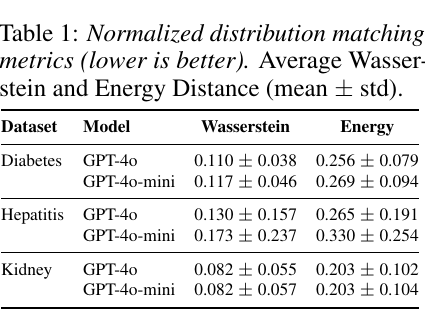
\includegraphics[width=\linewidth]{figures/actmed_table1_sampling.png}

    \vspace{0.5em}
    \footnotesize
    \textcolor{gray}{GPT-4o와 GPT-4o-mini 모두 비교적 낮은 distance를 보여,
    후보 검사 결과 샘플링이 실제 분포와 크게 어긋나지 않음을 확인.}
\end{column}

\end{columns}
\end{frame}


% ─────────────────────────────────────────────────────────────────────────────
% FRAME 8: 실험 결과 2
% ─────────────────────────────────────────────────────────────────────────────
\begin{frame}{실험 결과 2: 진단 정확도}
\centering
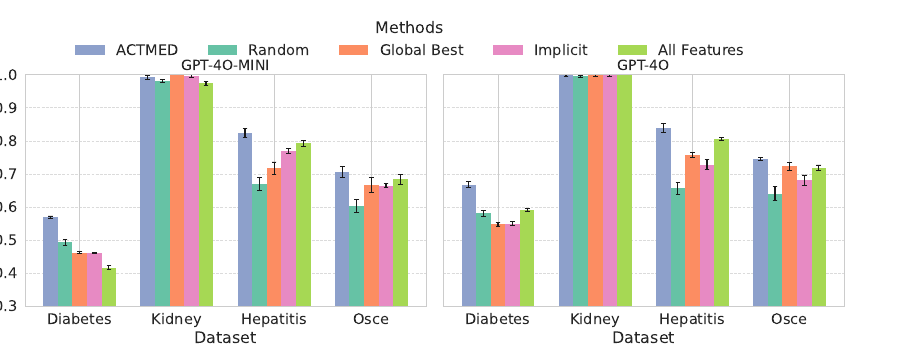
\includegraphics[width=0.86\textwidth]{figures/actmed_fig4_accuracy.png}

\vspace{0.4em}
\begin{block}{비교 설정}
\footnotesize
\begin{tabular}{lp{8.7cm}}
    \toprule
    방법 & 설정 \\
    \midrule
    All Features & 사용 가능한 모든 검사 항목을 관측한 상한선 설정 \\
    Random & 후보 검사 중 최대 3개를 무작위로 선택 \\
    Global Best & 환자별 정보를 보기 전, 태스크별 전역 최적 검사 3개를 고정 선택 \\
    Implicit & BED utility 없이 LLM에게 다음 검사를 직접 선택하게 하는 설정 \\
    \bottomrule
\end{tabular}
\end{block}

\vspace{0.2em}
\footnotesize
\textcolor{gray}{ACTMED는 BED utility를 사용해 환자별로 다음 검사를 선택하며, 각 환자당 최대 3개 검사만 사용.}
\end{frame}


% ─────────────────────────────────────────────────────────────────────────────
% FRAME 9: 한계 + 핵심 메시지
% ─────────────────────────────────────────────────────────────────────────────
\begin{frame}{한계 및 핵심 메시지}
\begin{columns}[c]

\begin{column}{0.48\textwidth}

    \begin{alertblock}{한계}
    \footnotesize
    \begin{itemize}\itemsep0.4em
        \item \textbf{데이터 규모}: 전체 약 1,000명\\
              \textcolor{gray}{실제 임상 적용 전 대규모 검증 필요}
        \item \textbf{이진 분류만 가능}: 복수 질환·동반 질환 미지원
        \item \textbf{Feature 수준만}: 모달리티 선택 불가\\
              \textcolor{gray}{(영상, 자유 텍스트, 유전체 미지원)}
        \item \textbf{고성능 LLM 의존}: GPT-4o급 필수;\\
              소형 모델 사용 시 프레임워크 전체 실패
        \item \textbf{계산 비용}: 후보 검사 수와 샘플 수에 비례해\\
              LLM 호출 수 증가
    \end{itemize}
    \end{alertblock}

\end{column}

\begin{column}{0.48\textwidth}

    \begin{block}{장점}
    \footnotesize
    \begin{itemize}\itemsep0.3em
        \item 임상 검사 선택을 BED 관점으로 정식화
        \item 태스크별 재학습 불필요 (제로샷)
        \item 단계별 투명한 추론 과정
        \item 임상의가 매 단계 검토·개입 가능
        \item 비용 인식적 검사 선택
    \end{itemize}
    \end{block}

    \vspace{0.4em}

    \begin{block}{핵심 메시지}
    \small
    ACTMED는 임상 진단을 \textbf{순차적 의사결정 문제}로 재정의.\\[0.4em]
    LLM이 BED의 \textbf{서로게이트}로 작동하여, 재학습 없이 환자별 최적 검사를 선택.\\[0.4em]
    \textcolor{gray}{현재 LLM은 자율 진단에는 \textbf{준비되지 않았지만}, 임상의를 의미있게 \textbf{보조}할 수 있음.}
    \end{block}

\end{column}

\end{columns}
\end{frame}


\end{document}
